\chapter{System Design}
\label{cha:system}
\vspace{0.4 cm} 

In this section, the methodology and the choices in the system design is presented. Starting by describing the components of the system with their functionalities (the blocks in the system architecture) and then explaining the working logic of the developed system. After this section, it will be clear which are the main parts of this system and how they cooperate to achieve the project goal.


\section{System architecture}
\label{sec:sysarc}
\vspace{0.2 cm} 

In a place of interest, there are people/users with their devices that are sending Wi-Fi packets, if they have the Wi-Fi device turned on. The purpose of our system is to exploit these packets to infer the number of people present. The system architecture of the developed system is shown in figure ~\ref{fig:architecture}. 
This is a distributed architecture, in fact, there are three main components on different platforms that cooperate over a communication network in order to achieve this goal.

\begin{figure}[h]
\centering 
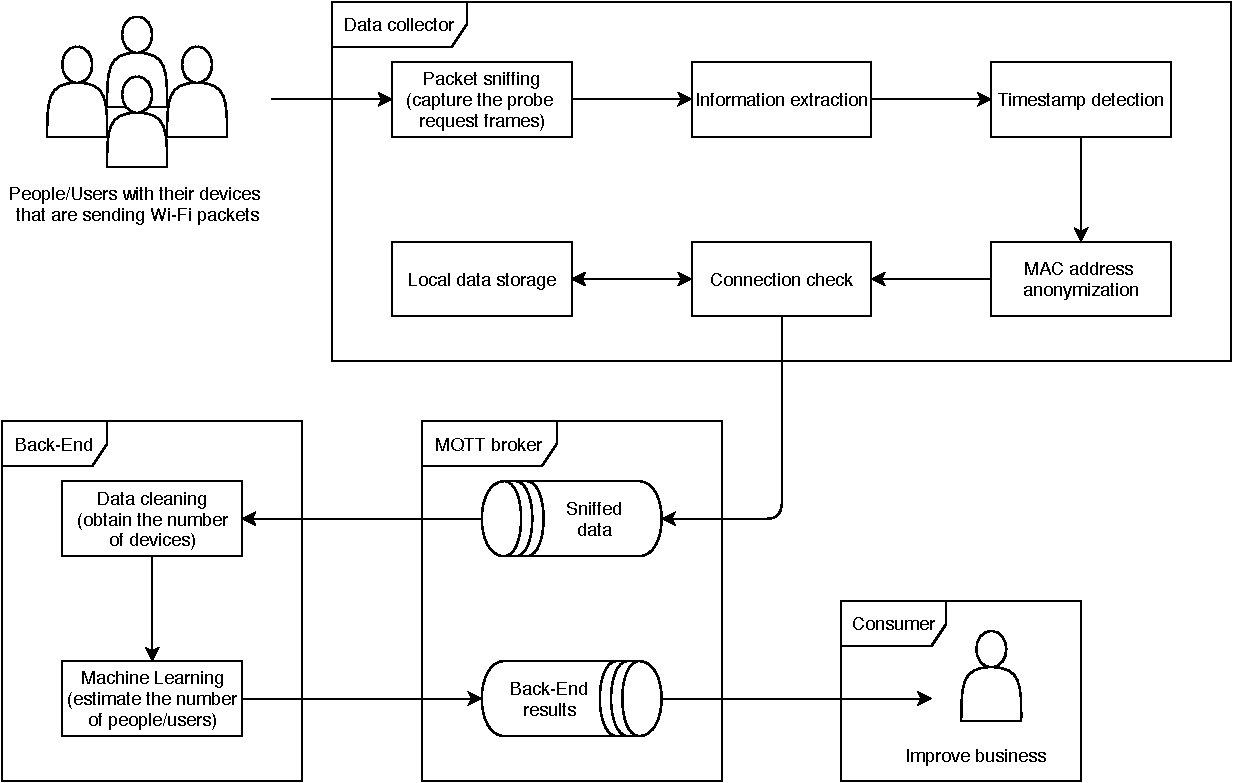
\includegraphics[width=0.9\textwidth]{images/architecture} 
\caption{Architecture of the proposed system.}
\label{fig:architecture}
\end{figure}

The first block of the system is a data collector (implemented on a Raspberry Pi 2B) which is located in the place of interest. It performs a preprocessing of the data (distributed work) with its functionalities: sniffing of Wi-Fi packets, capture the probe request frames; extract the useful information from these; detect the current timestamp; anonymize the MAC address using a hash function (no more privacy issues); check the internet connection; if there is no connection, save the data in the local storage; if there is a connection, publish the collected data to the dedicated queue (Collected data).

The system uses the MQTT protocol for data forwarding, an MQTT Broker (situated TBD, it must have a static IP address to be accessible, implemented using Mosquitto MQTT Broker) with 2 dedicated queues: one for the collected data (published by sensors and received by the subscribed Back-End) and the other one for the Back-End results (published by the Back-End and received by the subscribed consumer).

The Back-End (situated TBD, implemented on a pc or running on Google Colaboratory) deals with collected data cleaning -- (to be decided based on the use case: RSSI thresholding) remove random encounters (and randomized addresses are eliminated with this), make a blacklist to remove the ever-present devices or devices revealed too many times during the day and then get the number of devices present in the place of interest --, data analysis using Machine Learning -- fit the degree and the coefficients of the polynomial approximation using the trend and the seasonality of the number of devices detected to obtain the number of people present -- and publication of the results to the dedicated queue (Back-End results).

At the end of this processing, there is the consumer who receives the results of the Back-End, the number of people/users in the place of interest, and could use this information to improve his business.

This architecture is scalable, it could admit many sensors physically distributed in different environments for data collection, to provide a practical example some use cases are shown in figure ~\ref{fig:excases}.  It is important to locate them properly in the environments to cover all the areas of interest. All sensors publish data to the same MQTT broker and then all data is forwarded to the same Back-End. Cleaning and analysis will be performed according to the data source, each sensor will send data in its own reserved queue and will be analyzed adequately to the characteristics of the use case for which it was used. (in the end, they are sent to the respective consumer through an appropriate queue)

\begin{figure}[h]
\centering 
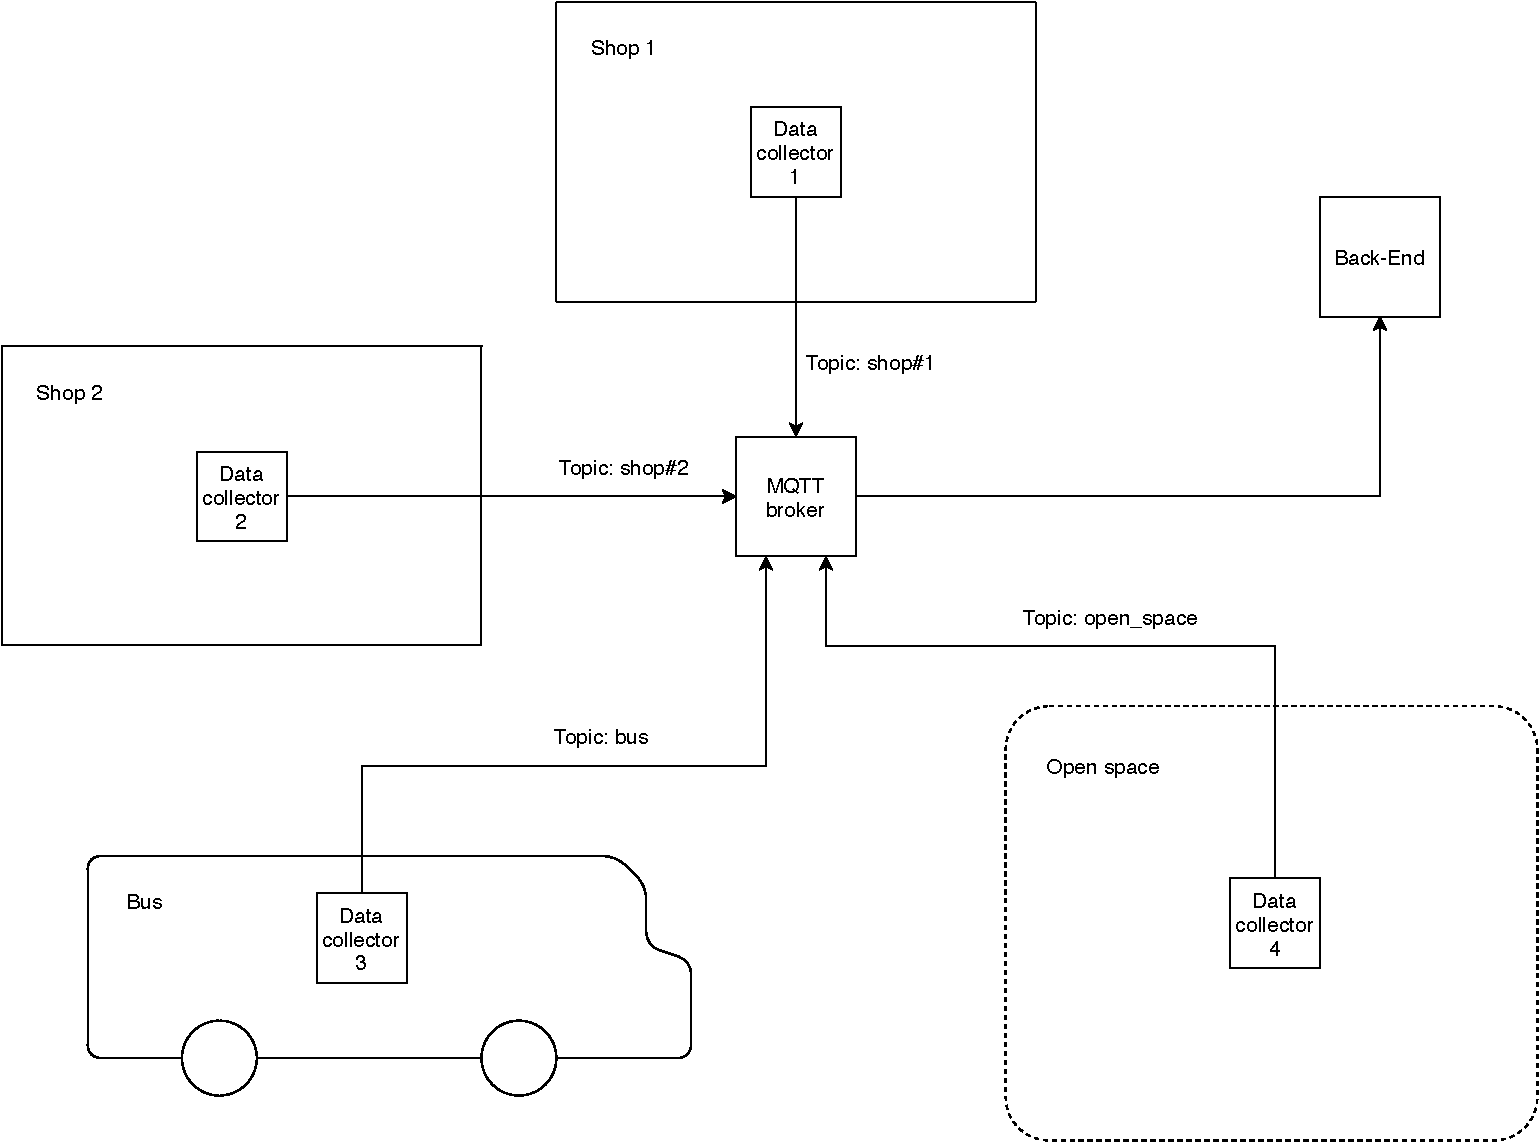
\includegraphics[width=0.9\textwidth]{images/excases} 
\caption{Presentation of a possible implementation with different use cases.}
\label{fig:excases}
\end{figure}


\section{Data collection}
\label{sec:collection}
\vspace{0.2 cm} 

The main block I worked on is the data collector. I developed the logic behind this block, with particular attention in the research of the connection and in the management of the data collected.

The flowchart representing the data collector logic is shown in figure ~\ref{fig:flowcollect}. When the data collector is turned on, the system searches for the connected Wi-Fi dongle and puts it in monitor mode to perform the packet sniffing. Initially, a packet counter is set = 0 and the actual time is saved. When a packet is received it checks if it is a probe request frame and if it is not, it is thrown away (using Scapy).
When a probe request frame is captured, the following information are extracted: RSSI, SSID (Service Set Identifier), MAC address, sequence counter. The timestamp when the packet was revealed is given by an RTC (Real Time Clock) board and together with the other information are saved temporarily in the RAM (Random Access Memory). The packet counter increases by one.

\begin{figure}[h]
\centering 
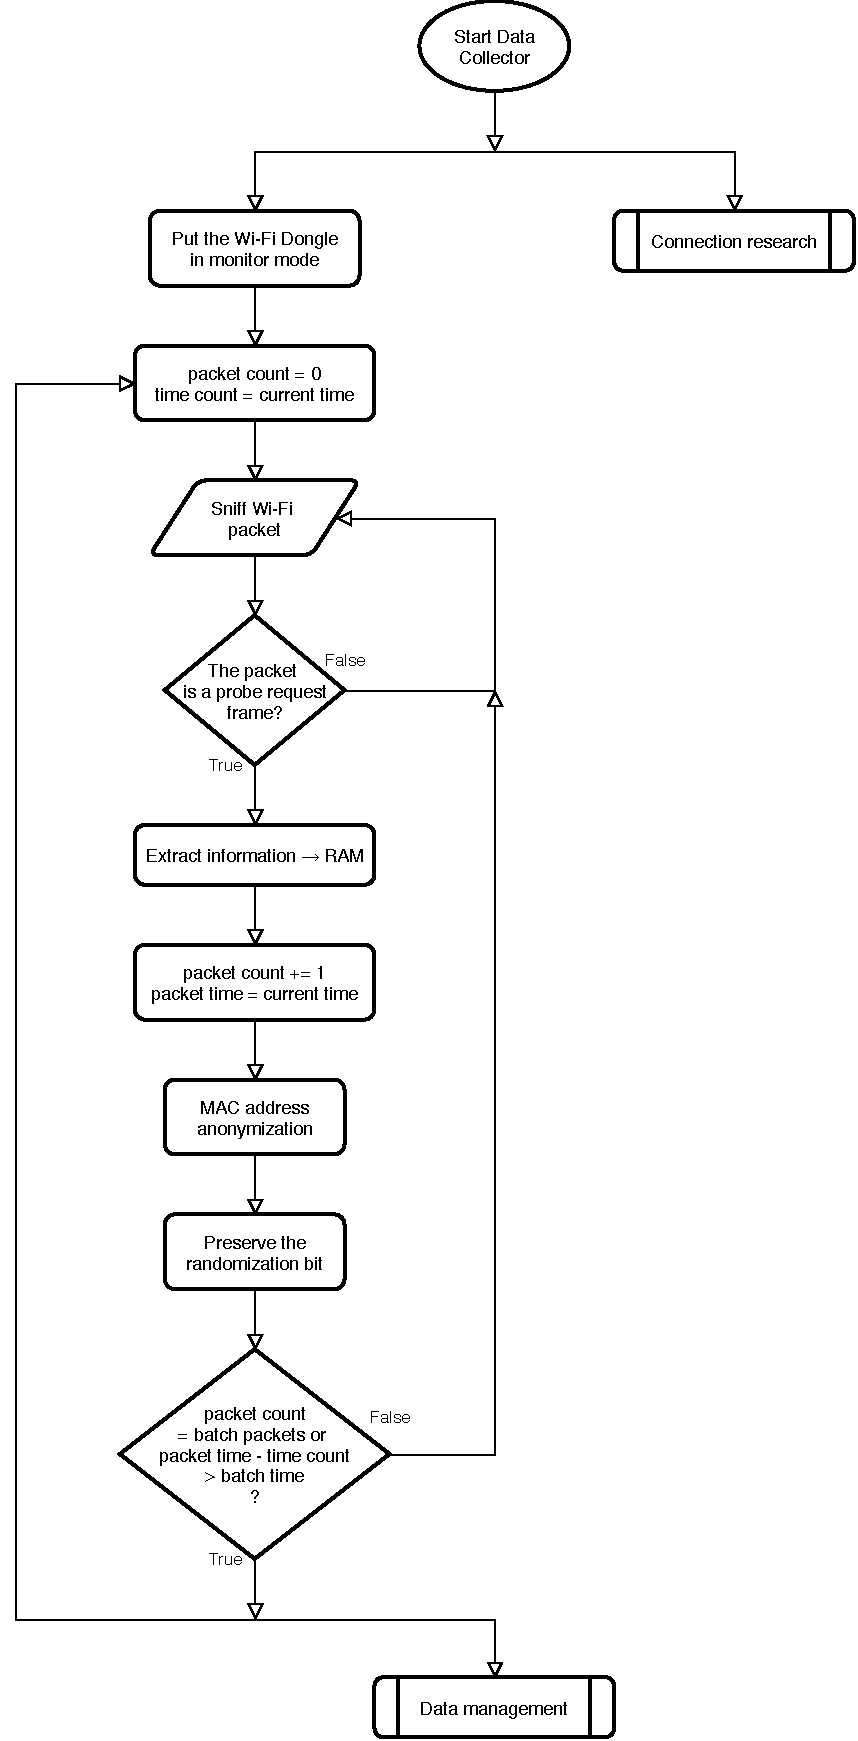
\includegraphics[width=0.7\textwidth]{images/flowcollect} 
\caption{Flowchart representing the data collector logic.}
\label{fig:flowcollect}
\end{figure}

After extracting the information, there is the anonymization of the MAC address to preserve the privacy of the users and comply with the GDPR. Anonymization is performed at this point in the architecture because then there are no more privacy problems, this work does not have to be done from the Back-End and for reasons of data security in case of a data breach during transmission.
This process consists of hashing the MAC address using BLAKE2s, an implementation of the BLAKE2  cryptographic hash function based on BLAKE  \footnote{https://blake2.net/} (BLAKE3 is faster but still under development). BLAKE2 is faster than MD5, SHA-1, SHA-2 and SHA-3, and provides security superior to SHA-2 and similar to that of SHA-3. BLAKE2 supports keying and salting, and can output digests from 1 up to 32 bytes for BLAKE2s. This hash function is the ideal for changing hash results every 24 hours or predefined time, simply modifying the key or adding a different value of salt. This is made for privacy reasons and to avoid tracing the MAC address although it is not the real one but always the same after hashing.

Among the information that can be extracted from the MAC address before performing the anonymization there are the OUI (Organizationally Unique Identifier), from which the manufacturer of the device can be identified, and the local bit, the 7\textsuperscript{th} bit of the MAC address, from which it can be seen whether the MAC address is randomized or not. If the anonymization changes the state of the bit, the previous state is forced/imposed to preserve this information on randomization, which can be used in the cleaning phase.

Once the pre-processing of the data is completed, we decided to process the collected data in batches and therefore there are to check 2 batch criteria, based on a maximum number of packets and a maximum time since the last batch transmission. These parameters have to be set according to the use case, once one of these is reached it is possible to decide what to do with this data by running the data management flowchart (shown in figure ~\ref{fig:flowdata}).
Higher values of the parameters allow us to avoid a continuous transmission of data and to fill the queue on the broker or in the lack of a connection, to open the file to save the data every time a packet is detected. On the other hand, choosing smaller values of the parameters reduces estimation delay, making the system more responsive. In our experiments, we used intermediate values with a maximum number of packets of 50 and a maximum time since the last batch transmission of 60 seconds, which is a good trade-off between congestion and transmission delay.

\begin{figure}[h]
\centering 
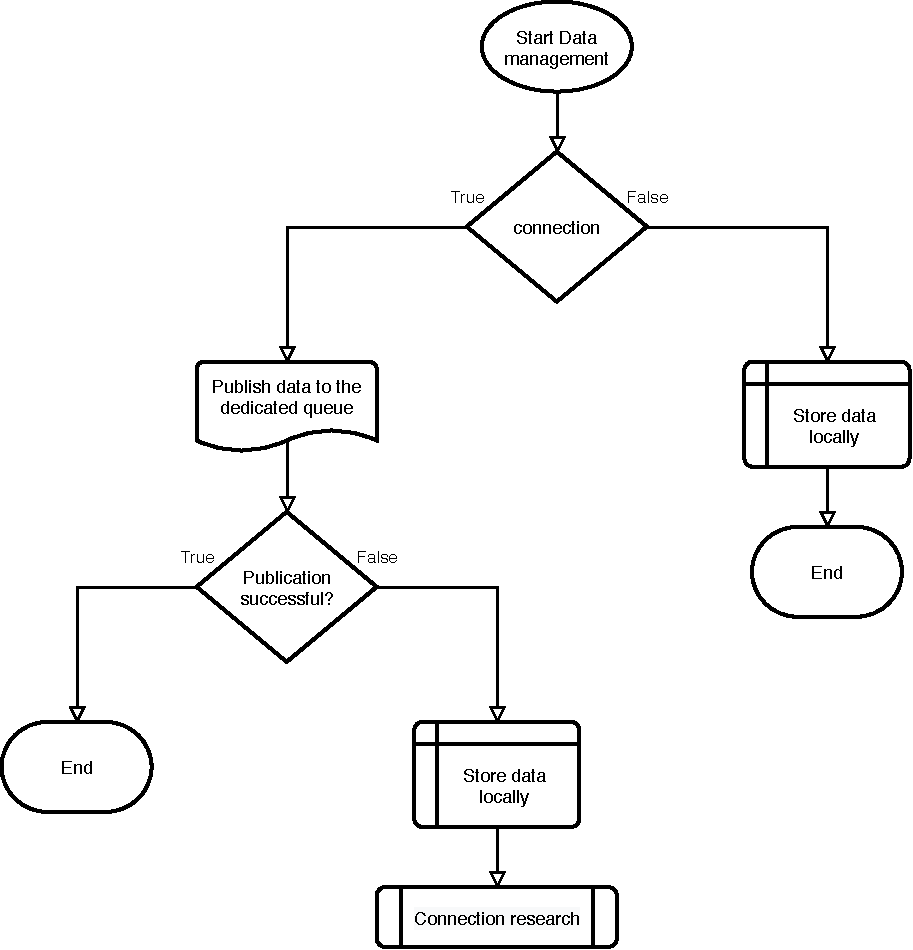
\includegraphics[width=0.7\textwidth]{images/flowdata} 
\caption{Flowchart representing the data management logic.}
\label{fig:flowdata}
\end{figure}

When the batch is ready, the algorithm for managing what to do with the data starts. If there is no connection, the collected data is stored locally (using json.dump()) to be sent later when a connection is found. After that, the data is deleted from the RAM.
Instead, if there is a connection with the MQTT broker, the collected data is published to the dedicated queue (Collected data, converted in a string using json.dumps() to be published). If the publication is successful, the data is deleted from the RAM. Otherwise, it is stored locally (using json.dump()), subsequently deleted from the RAM and finally the system searches again for a connection.

When the data collector is turned on, the system searches also for a connection with the MQTT broker. In figure ~\ref{fig:flowconnection} shows the flowchart explaining the logic behind this. Initially, the connection is set = False and the system checks whether the data collector has a peripheral with an IP address for Internet access.
When it has an IP address, a Paho MQTT Client with its credentials tries connecting to the MQTT broker. When the broker is reachable and accepts the client connection, the connection is set = True and if there is data stored locally, it can be published by running the flowchart for the publication of the stored data (shown in figure ~\ref{fig:flowstorage}).

\begin{figure}[h]
\centering 
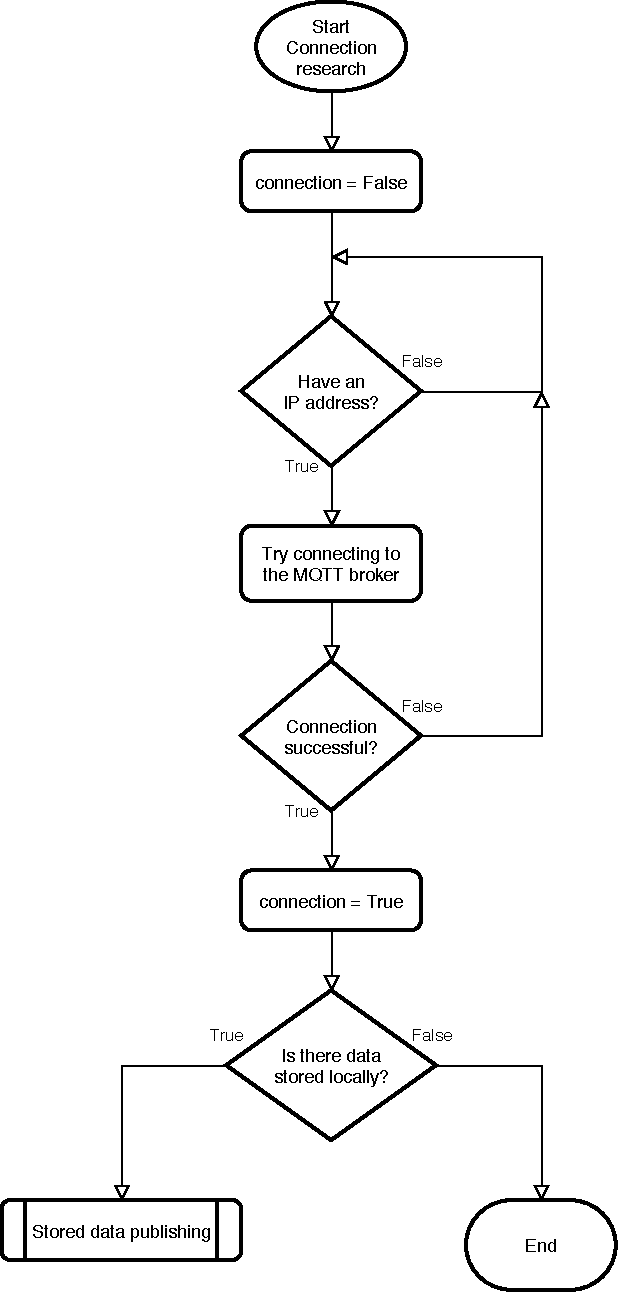
\includegraphics[width=0.7\textwidth]{images/flowconnection} 
\caption{Flowchart representing the connection research logic.}
\label{fig:flowconnection}
\end{figure}

\begin{figure}[h]
\centering 
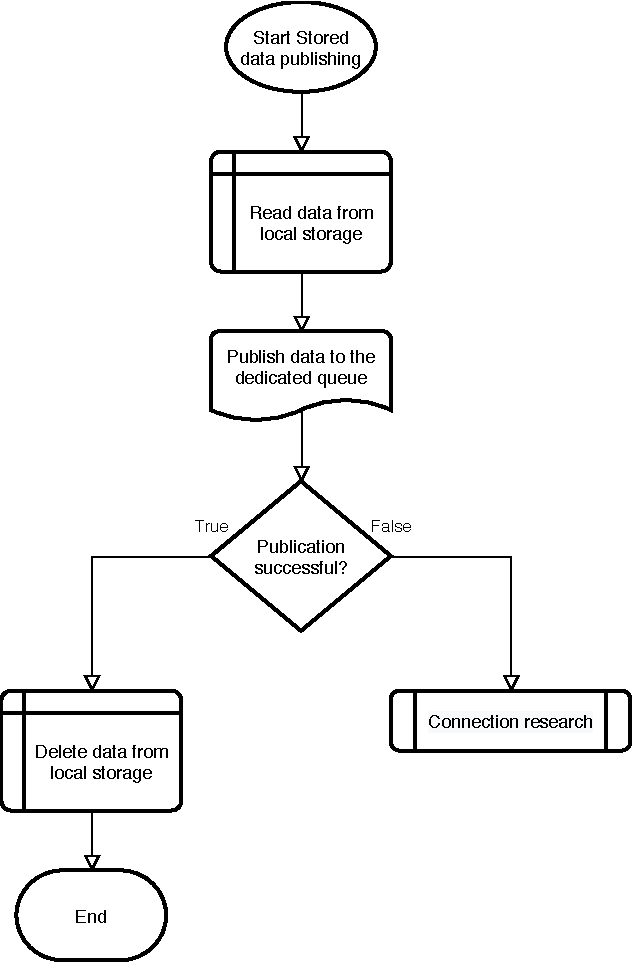
\includegraphics[width=0.7\textwidth]{images/flowstorage} 
\caption{Flowchart representing the stored data publishing logic.}
\label{fig:flowstorage}
\end{figure}

The data is read from the local storage (using json.loads()) and is published to the dedicated queue (Collected data, converted in a string using json.dumps() to be published). 
If the publication is successful, the data is deleted from the local storage. Otherwise, it remains stored locally and the system searches again for a connection.


\section{Data transfer}
\label{sec:transfer}
\vspace{0.2 cm} 

How the MQTT protocol has been used to forward the data and why I chose this protocol: MQTT functionalities and use of dedicated queues (one for the Collected data and the other one for the Back-End results), broker and protocol parameters setting (reasoning on publishing and QoS and other parameters).


\section{Data analysis}
\label{sec:analysis}
\vspace{0.2 cm} 

How the data has been analyzed: Back-End functionalities: processing data, clean data, analyze data using machine learning.
